\chapter{Study Area}
\label{ch:study_area}

The study area of this thesis is defined by the spatial coverage of the Google Open Buildings Dataset v3. This dataset mainly covers regions in the Global South and is therefore well suited for analysing building-footprint quality in areas where authoritative cadastral data is often incomplete or unavailable. Instead of focusing on one homogeneous region, five study areas were selected to represent different environmental, morphological and image-related conditions.

The selected areas are located in Liberia, Mexico, Nepal, Niger and Mozambique. They were chosen because they differ strongly in building form, roof material, settlement structure, vegetation cover, contrast between buildings and surrounding land cover, and the degree of tree occlusion. 

Table~\ref{tab:study_area_imagery_sources} summarizes the OpenAerialMap imagery used for the five study areas. All scenes are UAV-based orthomosaics with very high spatial resolution between 2 and 6\,cm. This high image resolution was important for the visual assessment of small buildings and for the patch-based refinement workflow.

\begin{table}[htb]
\centering
\caption{OpenAerialMap imagery used for the selected study areas.}
\label{tab:study_area_imagery_sources}
\footnotesize
\renewcommand{\arraystretch}{1.15}
\begin{tabularx}{\textwidth}{p{0.12\textwidth}X p{0.11\textwidth}p{0.10\textwidth}X p{0.11\textwidth}p{0.12\textwidth}}
\toprule
\textbf{Country} &
\textbf{OpenAerialMap scene} &
\textbf{Date} &
\textbf{Resolution} &
\textbf{Platform and sensor} &
\textbf{Image size} &
\textbf{License} \\
\midrule
Liberia &
Central Monrovia 1, uploaded by Frederick Mbuya; provider Uhurulabs &
2020-02-23 &
5\,cm &
UAV, S.O.D.A sensor &
413.02\,MB &
CC-BY 4.0 \\
Mozambique &
Nacala: Ontupaia, uploaded by \#MapeandoMeuBairro &
2022-03-31 &
5\,cm &
UAV, DJI Phantom 4 Pro V2.0 &
74.1\,MB &
CC BY-SA 4.0 \\
Nepal &
UAV Images of Banepa Municipality, uploaded by Cristiano Giovando; provider Geomatics Engineering Society &
2022-04-15 &
3\,cm &
UAV, DJI Mavic 2 Pro with 1-inch CMOS sensor &
2.76\,GB &
CC-BY 4.0 \\
Niger &
Orthomosaic Niamey, uploaded by Dr Barkawi Mansour; provider GeoMinds Africa &
2024-12-23 &
2\,cm &
UAV, DJI Mavic 3 Multispectral &
254.1\,MB &
CC-BY 4.0 \\
Mexico &
Centro Poblado Francisco I. Madero (Cintalapa), uploaded by Nicolas Vargas Ramirez; ENCiT UNAM field-practice orthomosaic &
2025-02-23 &
6\,cm &
UAV, DJI Mini 4K &
117.76\,MB &
CC BY-NC 4.0 \\
\bottomrule
\end{tabularx}
\end{table}

\begin{figure}[htb]
    \centering
    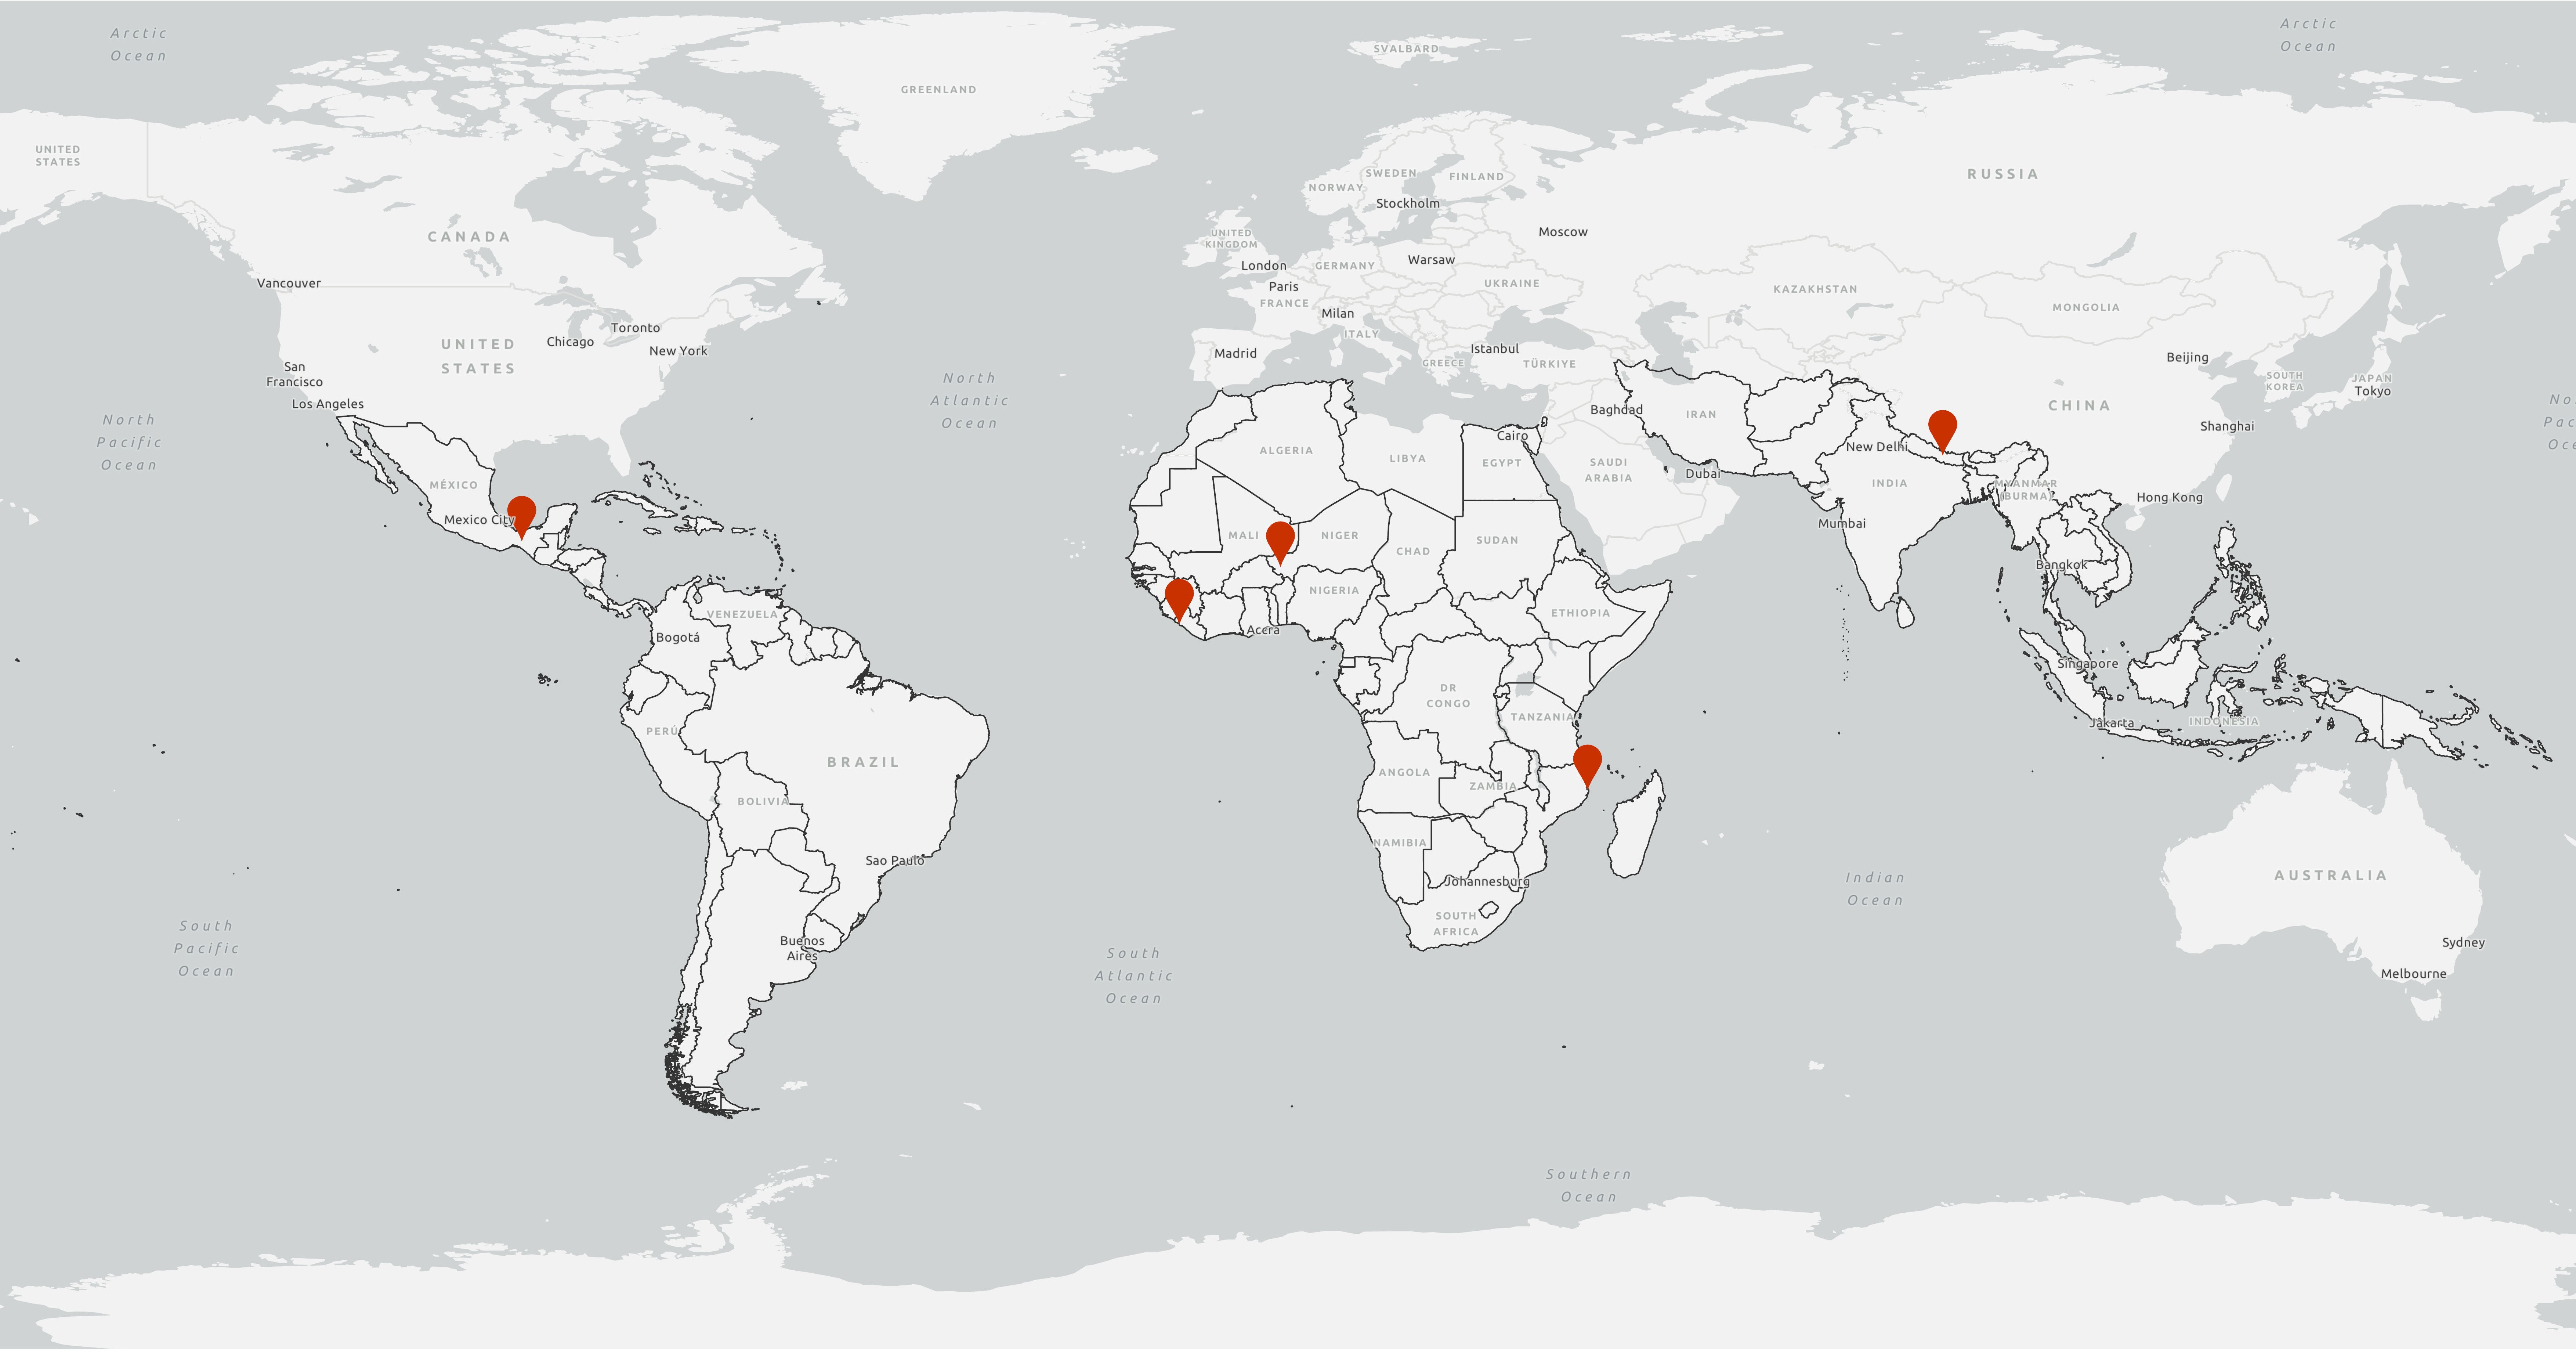
\includegraphics[width=\textwidth]{Franzelin_Master/img/googleopenbuildingextend.jpg}
    \caption{Spatial coverage of the Google Open Buildings Dataset v3 and selected study areas used in this thesis.}
    \label{fig:google_open_buildings_extent}
\end{figure}

The selected study areas are not intended to represent all possible global settlement types or biotopes. Rather, they provide a deliberately diverse test set for evaluating how robust the proposed workflow is under different real-world conditions. The focus is especially on cases where building footprints are difficult to extract or regularise because of low image contrast, irregular building shapes, vegetation occlusion or heterogeneous roof materials.

\begin{figure}[htb]
    \centering
    \includegraphics[width=\textwidth]{Franzelin_Master/img/study_area_examples_abcde.png}
    \caption{Spatial coverage of the Google Open Buildings Dataset v3 and selected study areas used in this thesis.}
    \label{fig:google_open_buildings_extent}
\end{figure}


\textbf{Mozambique:}

The study area in Mozambique is located at coordinates 40.708186°E, 14.568532°S in the village of Nacala. The scene represents a rural settlement structure with predominantly small, single-storey buildings distributed in a relatively sparse and unplanned arrangement. In contrast to more urbanised regions, there is almost no formal road infrastructure visible, and movement paths mainly consist of informal sandy tracks between the buildings. Most buildings have simple rectangular or slightly irregular footprints and are constructed from a mixture of corrugated metal roofs and organic roofing materials such as thatch or wooden structures. Especially the roofs made from natural materials often exhibit fuzzy or poorly defined edges in the imagery. Roof conditions vary strongly, ranging from bright reflective metal surfaces to darker weathered materials with low spectral contrast. The overall image contrast is relatively low due to the similarity between building materials and the surrounding sandy ground surface. Furthermore, the scene contains various small-scale objects and environmental noise, including vegetation patches, scattered trees, shadows, fences and small informal structures. Although tree occlusion is less dominant than in the Mexico study area, several buildings are still partially covered by vegetation. Compared to Niger, the settlement pattern appears slightly more heterogeneous in roof materials and object textures, while still maintaining mostly compact and relatively simple building geometries.

\textbf{Liberia:}

The study area in Liberia is located at coordinates 10.792940°W, 6.338041°N in the village of Sayon Town. In contrast to the more arid environments of Niger and Mozambique, this scene is characterised by a very strong spectral contrast between buildings and the surrounding landscape. The settlement is situated in a wetland-like environment with dense green vegetation and shallow water-covered areas, resulting in highly distinctive building-background separation. Most buildings are detached and distributed relatively irregularly across the landscape without a clearly structured street network. Instead of formal paved roads, only narrow informal paths and small access routes are visible. The buildings themselves are diverse rectangular structures with corrugated metal roofs; however, the roofing materials show strong heterogeneity in colour, brightness and condition. Many roofs consist of multiple differently coloured segments, repairs or extensions that have accumulated over time. In several cases, adjacent structures, shadows and small auxiliary constructions create visually complex boundaries. Furthermore, the settlement pattern appears to have developed organically over time, leading to irregular spacing and orientation between buildings. Compared to the other study areas, Liberia provides one of the clearest contrasts between buildings and surrounding land cover. 

\textbf{Mexico:}

The study area in Mexico is located at coordinates 93.757355°W, 16.803258°N in the village of Francisco I. Madero. Compared to the other selected study areas, this scene represents the most structured and urbanised settlement pattern. The buildings are generally aligned along a clearly defined road network with relatively wide streets and more organised parcel structures. This introduces stronger geometric regularity and orientation consistency than in the more organically developed settlements observed in Liberia or Mozambique. Most buildings are often larger and more complex than those in the African study areas. Many structures contain multiple connected building parts, roof extensions or inner courtyards, resulting in more complicated polygon geometries. Roof materials vary between concrete, metal and mixed surfaces. One of the defining characteristics of this study area is the very high degree of vegetation cover and tree occlusion. Numerous buildings are partially hidden beneath dense tree canopies, shadows or surrounding vegetation. In several cases, only fragments of rooftops remain visible in the imagery, which significantly complicates building extraction and footprint completion. Although the overall building-background contrast is higher than in the arid environments of Niger and Mozambique, the dense vegetation and the complex building forms introduces a different type of complexity.

\textbf{Nepal:}

The study area in Nepal is located at coordinates 85.521601°E, 27.640378°N in the village of Banepa. Among all selected study areas, this scene represents the morphologically most complex settlement structure. The buildings are arranged in an irregular and organically developed pattern that follows the local topography and terrain conditions. In contrast to the more planar settlements observed in Mexico or the African study areas, the terrain in Nepal is strongly influenced by slopes and terraced agricultural structures.The buildings themselves exhibit highly heterogeneous geometries with numerous extensions, attached substructures, courtyards and partially overlapping roof sections. Many roofs consist of multiple connected elements with different orientations and materials, resulting in complex polygon boundaries and several non-orthogonal edges. Roof materials vary strongly between metal sheets, concrete surfaces and mixed construction types. Some buildings also contain temporary or semi-open structures that further complicate the visual separation between building and non-building areas. In addition, the settlement includes narrow paths, retaining structures and terraced agricultural fields that introduce additional linear features and textures into the imagery.Vegetation cover and tree occlusion are comparatively limited in this scene, meaning that the primary challenge does not originate from occlusion but rather from the geometric and morphological complexity of the buildings themselves.


\textbf{Niger:}

The study area in Niger is located at coordinates 1.960051°E, 13.584270°N in the village of Saga Fondo. The scene represents a dense rural settlement in an arid environment characterised by dry soil surfaces, sparse vegetation and relatively low spectral contrast between buildings and the surrounding ground. Many structures exhibit similar colour tones to the bare soil, making the separation between buildings and background particularly challenging.Most buildings are small, compact and predominantly rectangular, often consisting of simple single-storey structures with flat concrete roofs or roofs made from local organic materials. Compared to the more morphologically complex buildings in Nepal or Mexico, the geometric forms are relatively regular and orthogonal. However, the dense arrangement of buildings and the close proximity between neighbouring structures frequently create ambiguous bo undaries and narrow gaps.The settlement pattern appears highly organic and informal, with narrow unpaved paths instead of structured road infrastructure. Numerous small-scale objects such as walls, containers, shadows, fences, temporary structures and household objects introduce significant visual noise into the imagery. Although vegetation cover is comparatively limited, several isolated trees and small shaded areas are present. The primary challenge in this study area is therefore not tree occlusion, but rather the combination of low contrast, dense settlement morphology and cluttered ground textures. 
